\documentclass[main.tex]{subfiles} % Subfile-Class



% ============================================================================== %
%                            Subfile document                                    %
% ============================================================================== %

\begin{document}

% Template

% ===================================
\section{Konzepterstellung Hinderniserkennung}~\label{appendix:Hinderniserkennung}

Dieser Abschnitt beschäftigt sich mit der Evaluation verschiedener
Distanzsensoren, welche die Anwesenheit eines Hindernisses detektieren sollen.

% ===================================
\subsection*{Anforderungen}

\paragraph{Distanz}
Die Streckenlängen belaufen sich laut \textit{FAQ} auf $0.5m \dots 2m$. Daher
muss zur Pylonen-Erkennung ein Sensor gefunden werden, welcher in eben diesem
Bereich plausible Werte zurückgeben kann. Bei Hindernissen wird davon
ausgegangen, dass sich diese in etwa in der Mitte der Streckenlänge befinden.
Ein entsprechender Sensor muss also auf mindestens $0.25 m$ genau Distanzen
detektieren können.

\paragraph{Genauigkeit}
Bei Pylonen muss lediglich die Anwesenheit detektiert werden, um entsprechende
Wegstrecken als nicht befahrbar zu bewerten. Eine Genauigkeit von $\pm 50 mm$
muss also ausreichend sein, um diese zu erkennen. Der Sensor, welcher Barrieren
erkennen sollte, muss dagegen ein wenig genauer arbeiten, da das Fahrzeug
zwecks Positionierung des Greifmechanismus gut ausgerichtet werden muss. Hier
wird also eine Detektion mit einer Genauigkeit von $\pm 10 mm$ angestrebt.

\paragraph{Gewicht und Baugrösse}
Das Gewicht ist in allen Fällen eine Einschränkung für jede Funktionseinheit.
Für die Sensorik ist dies zwar kein gravierender Faktor, da entsprechende
Bauteile in der Regel sehr leicht sind, nichtsdestotrotz gilt: Je kleiner und
leichter, desto besser.

\paragraph{Kosten}
Das Budget für die Entwicklung des Pfadfinders ist begrenzt. Daher soll ein
Budget von $30 CHF$ nicht überschritten werden beim Zusammenstellen dieser
Sensorik.

% ===================================
\subsection*{Konzeption}

\subsubsection*{Erkennen von Hindernissen und Pylonen}
Geplant ist, mit einem Sensor über die Hindernisse hinweg zu schauen, um so
Pylonen zu erkennen. Ein zweiter Sensor, welcher sich etwas tiefer befindet,
soll Hindernisbarrieren erkennen können. So wird über die Höhendifferenz
zwischen Pylonen und Hindernissen unterschieden.

\subsubsection*{Ultraschallsensor HC-SR04}
Der Ultraschallsensor HC-SR04 ist ein sehr einfacher, sehr günstiger Distanzsensor, welcher,
wie der Name bereits anmuten lässt, als Sonar Distanzen detektieren kann.
Seine Ansteuerung und Auswertung sind auf einem Mikroprozessor mit 2 GPIOs
sehr einfach umzusetzen und mit einer Messgenauigkeit von einigen $mm$ auch sehr genau.

Ein grosses Problem dieser Sensoren ist ihr grosser \textit{Messkegel}. Der
Winkel der ausgesendeten Schallwellen beträgt $15°$, was auf eine Distanz von
$2m$ bereits einen Messkegel von ca. $1 m$ Radius bedeutet.
Abbildung~\ref{fig:Genauigkeit_Ultraschallsensor} zeigt dies nochmals.

\begin{figure}[H]
    \centering
    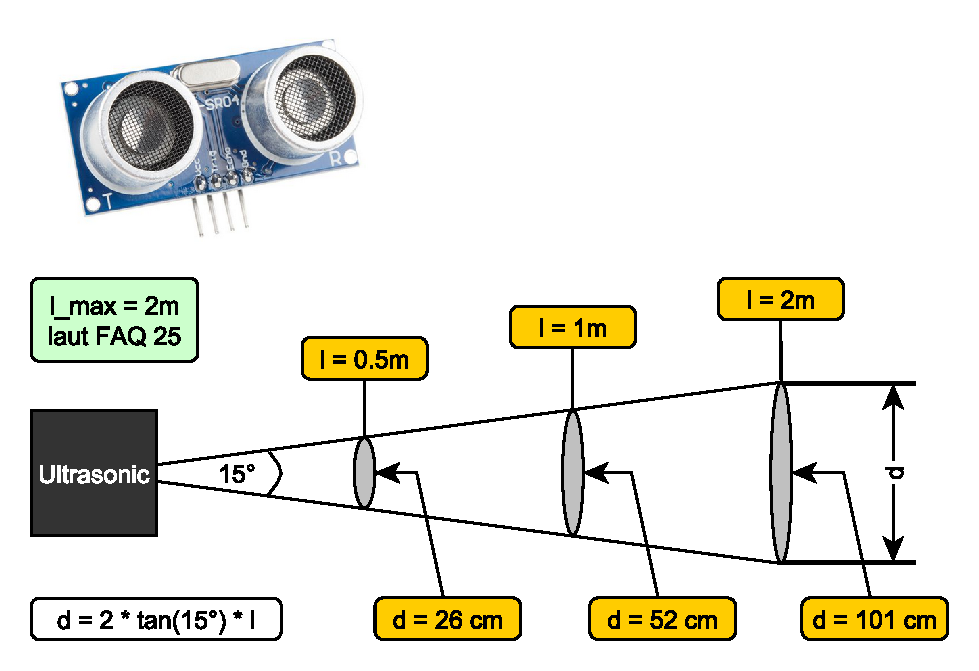
\includegraphics[width=0.75\linewidth]{./fig_Hinderniserkennung/Auslesegenauigkeit_Ultraschall.pdf}
    \caption{Messgenauigkeit Ultraschallsensor}~\label{fig:Genauigkeit_Ultraschallsensor}
\end{figure}

\subsubsection*{LIDAR}
Lidar-Sensoren sind tendenziell sehr teuer, zumindest wenn es darum geht
Sensoren, mit welchen das gesamte Umfeld erkannt werden kann, zu betrachten.
Auf dem Markt sind allerdings auch solche Sensoren erhältlich, welche ebenfalls
als LIDAR arbeiten, allerdings nur die direkte Distanz in eine einzige Richtung
detektieren können. Preislich bewegen sich diese in einem Rahmen von $20 - 30
    CHF$, was also noch innerhalb des Budgets für diese Sensorik liegen würde.
Ausgestrahlte Kegel sind bei Standard-Sensoren häufig $\approx 2°$ breit,
womit tatsächlich über ein Hindernis hinweg geschaut werden kann.
Abbildung~\ref{fig:Genauigkeit_LIDAR} zeigt dies nochmals.

\begin{figure}[H]
    \centering
    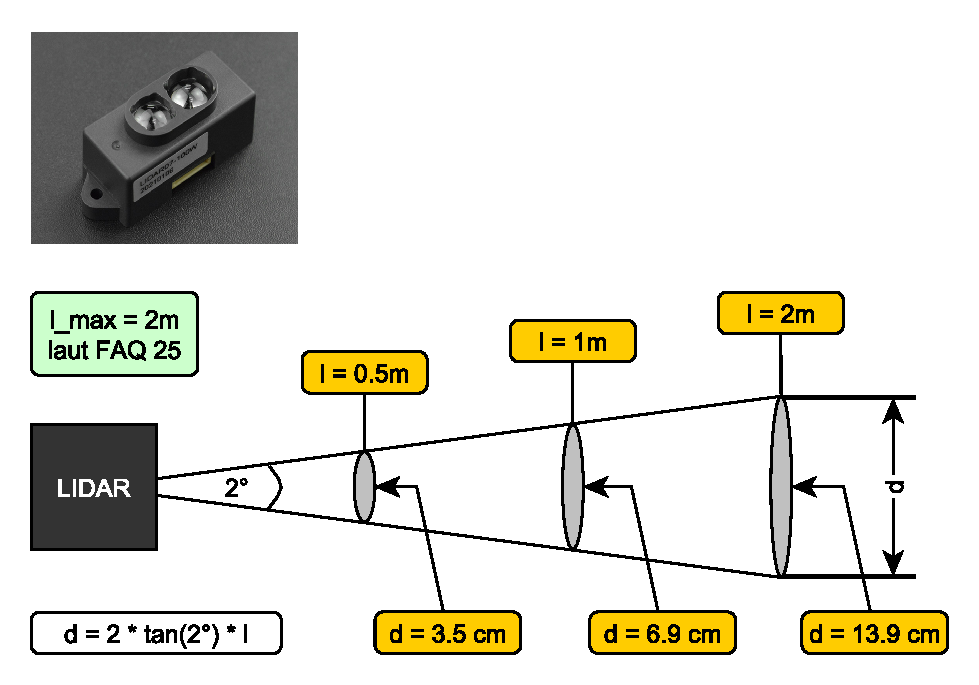
\includegraphics[width=0.75\linewidth]{./fig_Hinderniserkennung/Auslesegenauigkeit_LIDAR.pdf}
    \caption{Messgenauigkeit LIDAR}~\label{fig:Genauigkeit_LIDAR}
\end{figure}

Auf die Distanz sind diese Sensoren allerdings lediglich auf $20 mm - 30 mm$
sensitiv - eine grössere Auflösung wird allerdings auch nicht benötigt für
diese Anwendung. Der Messbereich üblicher Sensoren beginnt häufig erst bei $200
    mm - 300 mm$. Diese Sensoren können häufig sehr einfach über Registerzugriffe
via $I^2C$, UART oder SPI ausgelesen werden.

\subsubsection*{IR-Sensor}
Infrarotsensoren, wie der \textit{GP2Y0A02YK0F} von der Firma \textit{SHARP}
geben die gemessene Distanz als analoges Signal zurück. Sie sind sensitiv ab
einer Distanz von $200 mm$ bis auf $1500 mm$. Sie arbeiten auf der Basis eines
Infrarotlichtes - welches vom gegenüberliegenden Objekt reflektiert wird. Diese
Sensoren sind bereits ab $15 CHF$ auf dem Markt erhältlich. Aufgrund ihres sehr
eingeschränkten Messbereichs werden diese Sensoren nicht genauer untersucht -
da sie weder im Nahbereich für Hindernisse, noch im Fernbereich für Pylonen
eingesetzt werden könnten.

\subsubsection*{Lichtbarriere}
Eine Lichtbarriere, wie sie in Industriellen Anwendungen gerne eingesetzt wird,
kann zwar nicht eingesetzt werden, um direkt Distanzen zu Objekten zu messen, aber dafür,
die Anwesenheit eines Objektes sehr schnell und genau zu melden. Damit kann sichergestellt werden, dass sich das Hindernis zum entsprechenden Zeitpunkt ganz sicher an der richtigen Position vor dem Fahrzeug befindet.

Ein Team-Mitglied kann aus seinem beruflichen Umfeld auf solche Lichtbarrieren
der Firma \textit{SICK} zurückgreifen - wodurch diese folglich sehr günstig für
dieses Projekt erhältlich sind. Abbildung~\ref{fig:SICK_Sensor} zeigt eine
solche Lichtschranke.

\subsubsection*{Kamera und Bilderkennung}
Der Roboter wird in jedem Fall eine Kamera verbaut haben, da mit dieser
versucht werden soll, verschiedene Linienabgänge zu detektieren. Mit dieser Kamera
ist es durchaus ebenfalls möglich, Hindernisse zu erkennen. Kameras sind allerdings im Folgemodul noch
genauer zu untersuchen, gerade in Bezug auf Störempfindlichkeit bei unterschiedlichen Lichtverhältnissen.

\begin{figure}[H]
    \centering
    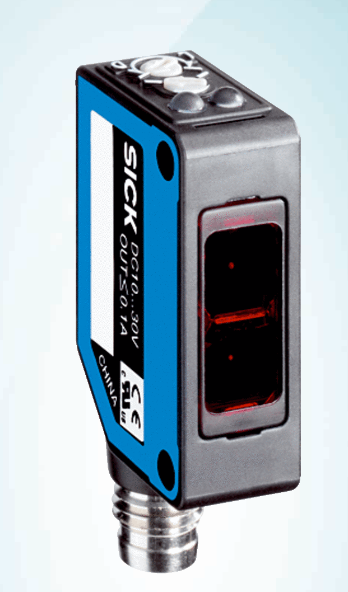
\includegraphics[width=0.25\linewidth]{./fig_Hinderniserkennung/SICK_Lichtschranke.png}
    \caption{Lichstchranke SICK}~\label{fig:SICK_Sensor}
\end{figure}

\subsubsection*{Fazit und Entscheidung der Konzeptphase}

Um Pylonen in der Ferne zu erkennen, wird ein LIDAR eingesetzt. Genauer gesagt
soll der Sensor \textit{TFLuna} von \textit{Benewake} eingesetzt werden. Er
bietet eine hohe Resistenz gegen Sonneneinstrahlung, einen kleinen Messkegel
und einen sehr überzeugenden Preis. Dieser Sensor ist in
Abbildung~\ref{fig:TFLuna} gezeigt.

\begin{figure}[H]
    \centering
    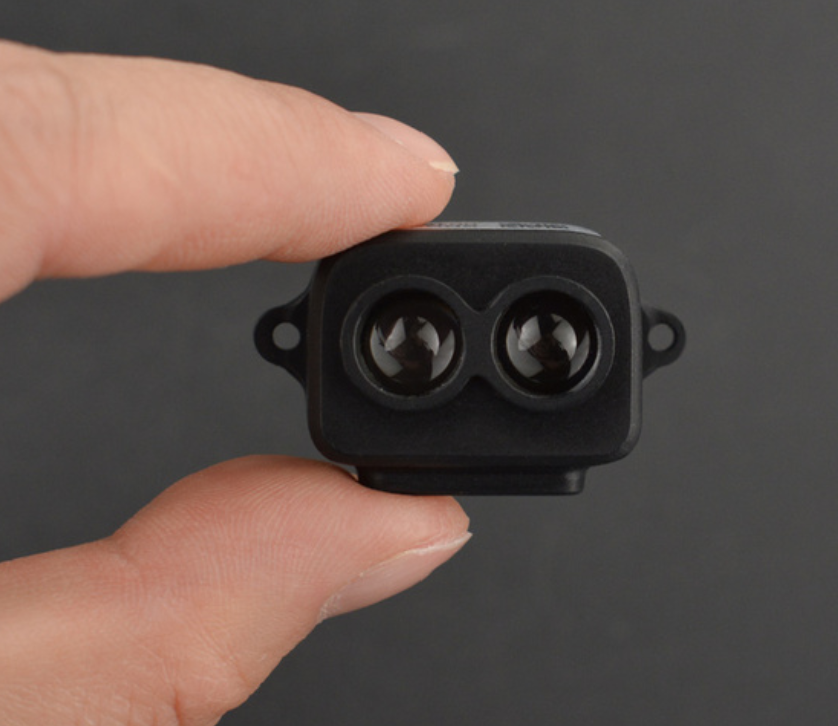
\includegraphics[width=0.25\linewidth]{./fig_Hinderniserkennung/TFLuna_Benewake.png}
    \caption{TFLuna LIDAR}~\label{fig:TFLuna}
\end{figure}

In einem ersten Prototypenaufbau werden mehr Sensoren eingesetzt als in Zukunft
vermutlich benötigt werden. So soll grundsätzlich die Anwesenheit eines
Hindernisses in der Position, in der es gegriffen werden kann, anhand einer
Lichtschranke detektiert werden. Trotzdem wird redundant ein Ultraschallsensor
auf Höhe der Hindernisse vorgesehen, welcher im Nahbereich bis zu $0.5m$
Hindernisse erkennen soll. Dadurch kann frühzeitig der Bremsvorgang eingeleitet
werden. Falls sich bei Versuchen mit dem Prototyp herausstellt, dass auch die
Positionierung des Hindernisses anhand des Ultraschallsensors genau bestimmt
werden kann, wird auf die zusätzliche Lichtschranke verzichtet. Parallel dazu
werden Auswertemöglichkeiten mit der Kamera weiter untersucht, womit ebenfalls
die Orientierung und Position des Hindernisses ermittelt werden kann.
Abbildung~\ref{fig:Hinderniserkennung} zeigt das erste angestrebte Konzept
nochmals skizziert.

\begin{figure}[H]
    \centering
    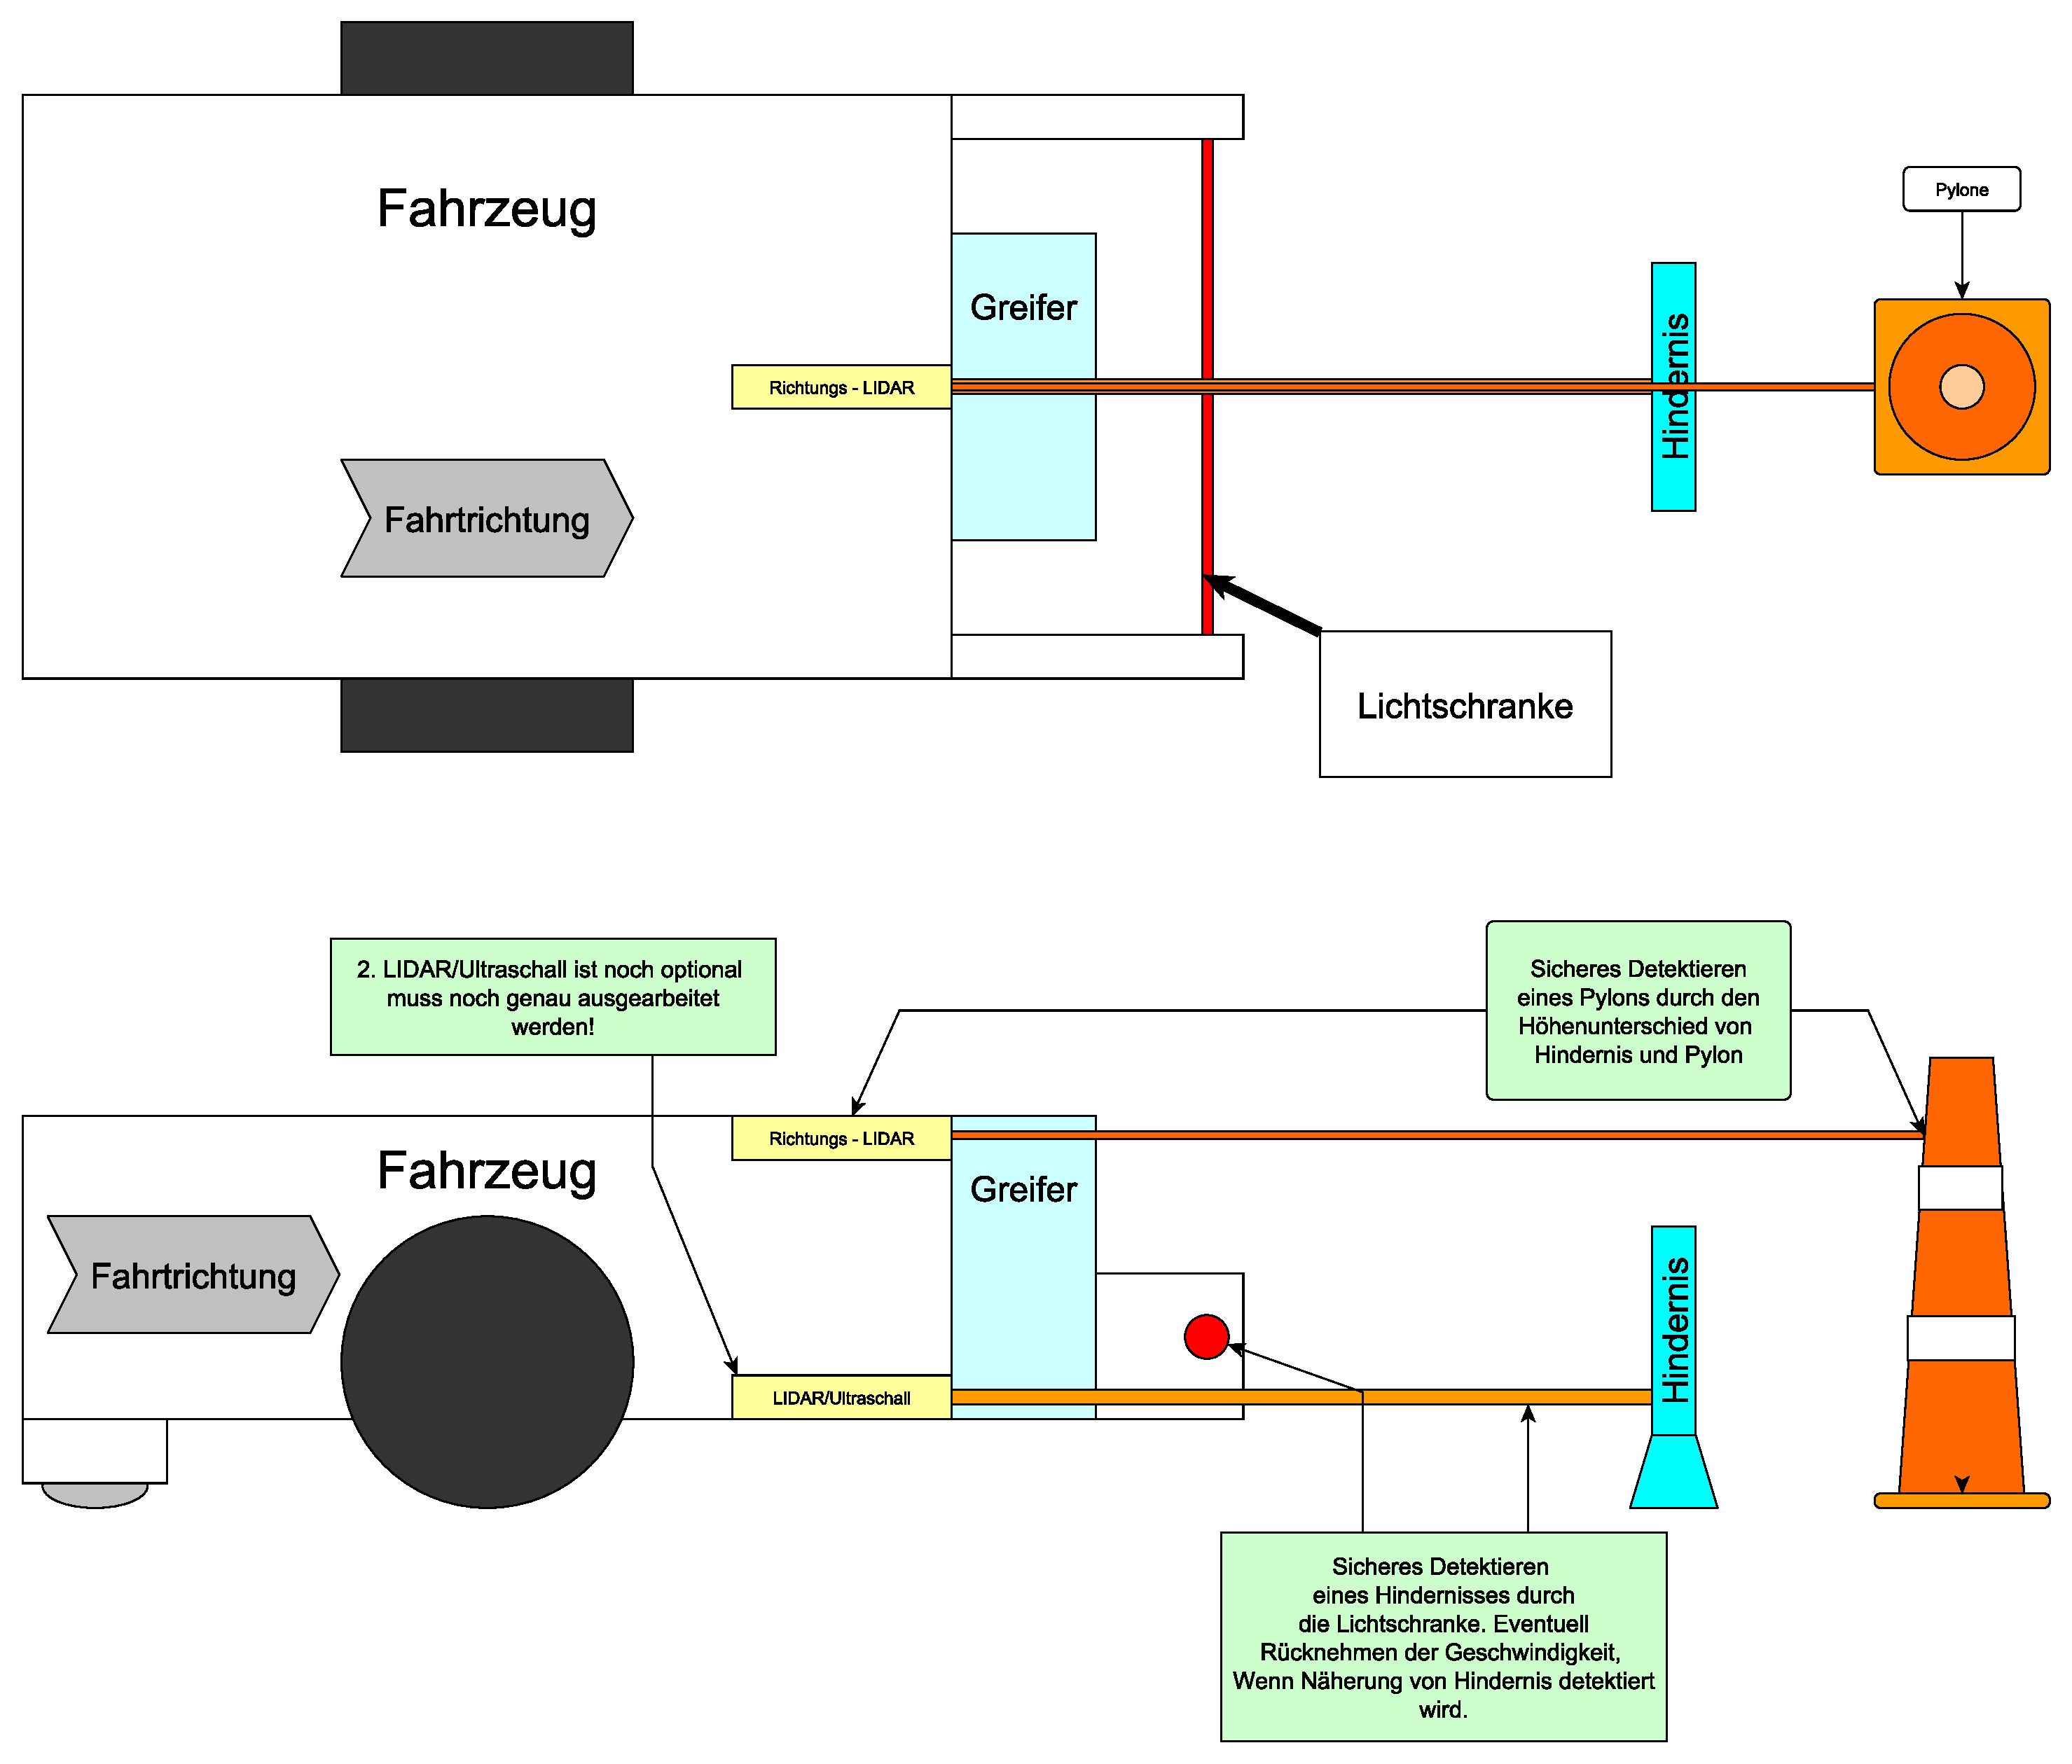
\includegraphics[width=0.75\linewidth]{./fig_Hinderniserkennung/Konzept_Hinderniserkennung.pdf}
    \caption{Konzept Hinderniserkennung}~\label{fig:Hinderniserkennung}
\end{figure}

\end{document}

